%%%%%%%%%%%%%%%%%%%%%%% file template.tex %%%%%%%%%%%%%%%%%%%%%%%%%
%
% This is a general template file for the LaTeX package SVJour3
% for Springer journals.          Springer Heidelberg 2010/09/16
%
% Copy it to a new file with a new name and use it as the basis
% for your article. Delete % signs as needed.
%
% This template includes a few options for different layouts and
% content for various journals. Please consult a previous issue of
% your journal as needed.
%
%%%%%%%%%%%%%%%%%%%%%%%%%%%%%%%%%%%%%%%%%%%%%%%%%%%%%%%%%%%%%%%%%%%
%
% First comes an example EPS file -- just ignore it and
% proceed on the \documentclass line
% your LaTeX will extract the file if required
\begin{filecontents*}{main.pdf}
%!PS-Adobe-3.0 EPSF-3.0
%%BoundingBox: 19 19 221 221
%%CreationDate: Mon Sep 29 1997
%%Creator: programmed by hand (JK)
%%EndComments
gsave
newpath
  20 20 moveto
  20 220 lineto
  220 220 lineto
  220 20 lineto
closepath
2 setlinewidth
gsave
  .4 setgray fill
grestore
stroke
grestore
\end{filecontents*}
%
\RequirePackage{fix-cm}
%
%\documentclass{svjour3}                     % onecolumn (standard format)
%\documentclass[smallcondensed]{svjour3}     % onecolumn (ditto)
\documentclass[smallextended]{svjour3}       % onecolumn (second format)
%\documentclass[twocolumn]{svjour3}          % twocolumn
%
\smartqed  % flush right qed marks, e.g. at end of proof
%
\usepackage{graphicx}
\usepackage{listings}
\usepackage{hyperref}
%\lstset{
%  basicstyle=\small\ttfamily,
%  columns=fullflexible,
%}

\lstset{language=C++,
 basicstyle=\ttfamily\scriptsize, %aboveskip={-5ex},
 columns=fullflexible,
%basicstyle={\ttfamily\singlespacing},aboveskip={-4ex},
 keywordstyle=\color{blue}\ttfamily,
 stringstyle=\color{red}\ttfamily,
 commentstyle=\color{cyan}\ttfamily,
 captionpos=t,
  %numbers=none, %left,
 numbers=left,
  %numberstyle=\scriptsize,
  %stepnumber=1,
  %numbersep=6pt,
  showstringspaces=false,
  breaklines=true,
  frame=lines,
  otherkeywords={[[,]],::},
  emph={rpr,kernel,target,in,out,pipeline,stream,farm,pipe,map,sync,async, rprmv, base, split, unroll, Pipeline, Farm, parallel_execution_ff},
  emphstyle={\color{magenta}\bfseries}
}

\usepackage{pgfplots}
\usepackage{xspace}
\usepackage{subfigure}
%\usepackage{subcaption}



%
% \usepackage{mathptmx}      % use Times fonts if available on your TeX system
%
% insert here the call for the packages your document requires
%\usepackage{latexsym}
% etc.
%
% please place your own definitions here and don't use \def but
% \newcommand{}{}
%
% Insert the name of "your journal" with
% \journalname{myjournal}
%
\begin{document}

\title{Refactoring GrPPI: Generic Refactoring for Generic Parallelism in C++}%\thanks{Grants or other notes
%about the article that should go on the front page should be
%placed here. General acknowledgments should be placed at the end of the article.}


%\titlerunning{Short form of title}        % if too long for running head

\author{Christopher Brown         \and
        Vladimir Janjic \and 
        Kenneth MacKenzie \and
        Adam Barwell \and
        Imre Pechan
}

%\authorrunning{Short form of author list} % if too long for running head

\institute{C. Brown, V. Janjic, A. Barwell \at
              School of Computer Science \\
              University of St Andrews \\
              UK. \\
              \email{cmb21,vj32,adb23@st-andrews.ac.uk}           %  \\
%             \emph{Present address:} of F. Author  %  if needed
           \and
            K. Mackenzie \at
                IOHK \\
              \email{thingy...} 
         \and
                I. Pechan \at
               EvoPro Innovation \\
              Hungary. \\
              \email{Pechan.Imre@evopro.hu}
}

\date{Received: date / Accepted: date}
% The correct dates will be entered by the editor


\maketitle

\begin{abstract}
Insert your abstract here. Include keywords, PACS and mathematical
subject classification numbers as needed.
\keywords{First keyword \and Second keyword \and More}
% \PACS{PACS code1 \and PACS code2 \and more}
% \subclass{MSC code1 \and MSC code2 \and more}
\end{abstract}

\section{Introduction}
\label{intro}

\noindent
The scale of parallelism in modern hardware systems is increasing at a very fast rate, with 72-core systems available off-the-shelf even in the embedded market\footnote{\url{http://www.mellanox.com/page/products_dyn?product_family=238&mtag=tile_gx72}}. At the same time, such systems are becoming increasingly heterogeneous, integrating GPUs, FPGAs, DSLs and other specialised processors within the same chip. This large scale of parallelism and heterogeneity of systems makes programming modern parallel hardware very difficult, often requiring a combination of different (and usually complex) programming models (e.g.~POSIX threads for the central multicore processor and OpenCL for GPUs), coupled with careful manual tuning, to achieve good performance. 

Parallel patterns~\cite{Asanovic:2009:VPC} have been recognised as an excellent compromise between the ease of programming and ability to generate efficient code for large-scale heterogeneous parallel architectures. They have been endorsed by several major IT companies, such as Intel and Microsoft as a means of programming parallel applications. This has given rise to a multitude of parallel pattern libraries, most of which are incompatible with one another and each of which usually has specific advantages (and disadvantages) over the others. GrPPI~\cite{DBLP:journals/concurrency/AstorgaD0G17} represents one of the first attempts at a uniform interface to parallel patterns, based on C++ template programming that allows the generation of target code for different pattern libraries. The code in Figure~\ref{fig:grppiExample} shows a snippet of code for a \emph{farm} pattern that targets both OpenMP and Intel TBB pattern libraries. While GrPPI makes the patterned code much easier to write, and also significantly eases rewriting of the code to use different pattern libraries, transforming sequential code to use GrPPI is still a very non-trivial task. The programmer needs to first ensure that it is \emph{safe} (in terms of unexpected side effects and race conditions) to transform the sequential code into its equivalent parallel implementation, and, secondly, to transform loops of the sequential code into calls to the appropriate patterns. 

\begin{figure}[t]
\centering
\subfigure[OpenMP] {
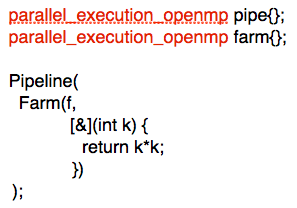
\includegraphics[width=0.35\textwidth]{GrPPIExampleOpenMP.png}
 \label{fig:grppiExampleOpenMP}}
 \subfigure[Intel TBB] {
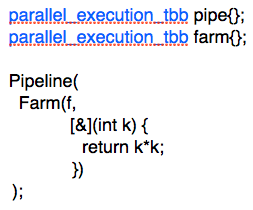
\includegraphics[width=0.30\textwidth]{GrPPIExampleTBB.png}
 \label{fig:grppiExampleTBB} 
  }
\caption{Example of the \emph{farm} pattern in GrPPI targetting OpenMP and TBB pattern libraries. Highlighted are parts of the code that differ between the two versions.}
\label{fig:grppiExample}
\end{figure}

This paper describes \emph{software refactorings} to introduce GrPPI patterns into the sequential code. These refactorings, implemented in the ParaFormance toolset for developing and maintaining parallel programs, provide a semi-automatic way of transforming sequential C++ code into its parallel patterned counterpart. The programmer is only required to insert simple annotations in the code to denote the parts that are, possibly, amenable to patterned parallelisation. We also describe \emph{safety checking} mechanisms that ensure the parts of the code annotated by the programmer are, indeed, safe to be transformed into patterns. Safety checking is based on s static analysis of the loops in the code to ensure that the loops are free of side effects (or, alternatively, that the side effects can be safely eliminated), that the order in which loop iterations are executed does not change the code semantics, etc. 

The specific research contributions of this paper are:
\begin{enumerate}
    \item we describe novel refactorings to introduce \emph{farm} and \emph{pipeline} parallelism, based on GrPPI interface, into the sequential C++ code, implemented as part of the \emph{ParaFormance} refactoring tool-set;
    \item we describe static analysis mechanisms that ensure the sequential code is safe for the application of refactorings to introduce patterned parallelism;
    \item we demonstrate the effectiveness of the refactorings and safety checking mechanisms on a number of benchmarks and real world examples, showing good speedups over the sequential code of the patterned code generated using the refactorings.
\end{enumerate}



%\subsection{Contributions}

\section{Background}
\label{background}

\subsection{Parallel Patterns}
%\begin{itemize}
%\item What are parallel patterns
%\item Some common patterns
%  \item Benefits of using patterns
%  \item Relevant pattern libraries (Open MP, Intel TBB...)
%\end{itemize}



\noindent
\emph{Parallel patterns} are a high-level abstraction for representing classes of computations that are similar in terms of their parallel structure, but different in terms of problem-specific operations. A typical example of a parallel pattern is a \emph{parallel map}, where the same operation is applied to a set of independent inputs in parallel. Regardless of whether the actual operation is, for example, multiplying a matrix by a vector or processing a pixel of an image, the parallel structure of the computation will be the same. Parallel Patterns are typically implemented as library functions, which handle creation, synchronisation and communication between the parallel threads, while the problem-specific (often sequential) computations are provided as the pattern parameters. In this paper, we restrict ourselves to two classical parallel patterns, which we believe to be the most common. Note that the technique described in this paper can be further generalised to include the full tractable set of parallel patterns.
\begin{itemize}
    \item The farm pattern models a data parallel computation, where a single computational worker, $f$, is applied to a set of independent inputs, $x_{1}, ..., x_{n}$. The parallelism arises from applying the worker, $f$, to different input elements at the same time in parallel. 
    \item The pipeline pattern models a parallel pipeline. Here, a sequence of functions, $f_{1}, f_{2}, ..., f_{m}$ are applied, to a stream on independent inputs, $x_{1}, ..., x_{n}$. The output of $f_{i}$ becomes the input to $f_{i+1}$, so that the parallelism arises from executing $f_{i+1}(f_{i}(...f_{1}(x_{k})...))$ in parallel with $f_{i}(f_{i-1}(...f_{1}(x_{k+1})...))$.
\end{itemize}

%The benefits of using parallel patterns lie in clear separation between sequential and parallel parts of the code and high-level description of the underlying parallelism, which makes the patterned applications much easier to maintain, change and adapt to new architectures. For these reasons, they have been endorsed by most of the top IT companies, who have their own pattern libraries, such as Microsoft PPL~\cite{ppl} and Intel Thread Building Blocks~\cite{tbb}. In addition to that, there are also many popular open-source pattern libraries, such as OpenMP~\cite{openmp} and FastFlow~\cite{openmp}.

\subsection{Refactoring and the ParaFormance Tool-chain}

\noindent
\emph{Refactoring} is the process of changing the structure of a program while preserving
its functional semantics in order, for example, to increase code quality, programming
productivity and code reuse. The term refactoring was first introduced by Opdyke in his PhD thesis in 1992~\cite{opdyke}, and the concept goes at least as far back as the fold/unfold system proposed by Burstall and Darlington in 1977~\cite{darlington77}. In our case, refactorings are source-to-source transformations of the code that are performed \emph{semi-automatically}, under the programmers guidance and possibly with his input. 

%
%
%
%\subsection{ParaFormance}

ParaFormance (\url{http://www.paraformance.com}) is a refactoring tool-suite developed at the University of St Andrews that refactors C and C++ programs into parallel versions. It targets a number of different back-ends, including FastFlow, Intel Thread Building Blocks (TBB), OpenMP and GRPPI. It has a number of unique features and is integrated as a plugin into both Eclipse and Microsoft Visual Studio, presenting a menu of various options to its users. ParaFormance provides \emph{semi-automated refactorings} to introduce parallel patterns into sequential code; \emph{safety checking} features to find, statically, parallelism related bugs, such as race-conditions, deadlocks and memory collisions; and \emph{pattern discovery}, to find the hotspots in the program that are suitable for parallelism. All refactorings applied to source code in ParaFormance are fully undoable. Furthermore, all operations in ParaFormance come with a full preview feature, enabling users to see the result of the transformation before applying it. Figure~\ref{fig:paraformance1} gives a screenshot of the ParaFormance tool integrated into Visual Studio. The refactorings presented in the this paper are implemented in ParaFormance as a plugin for both Visual Studio and Eclipse.

\begin{figure}
    \centering
    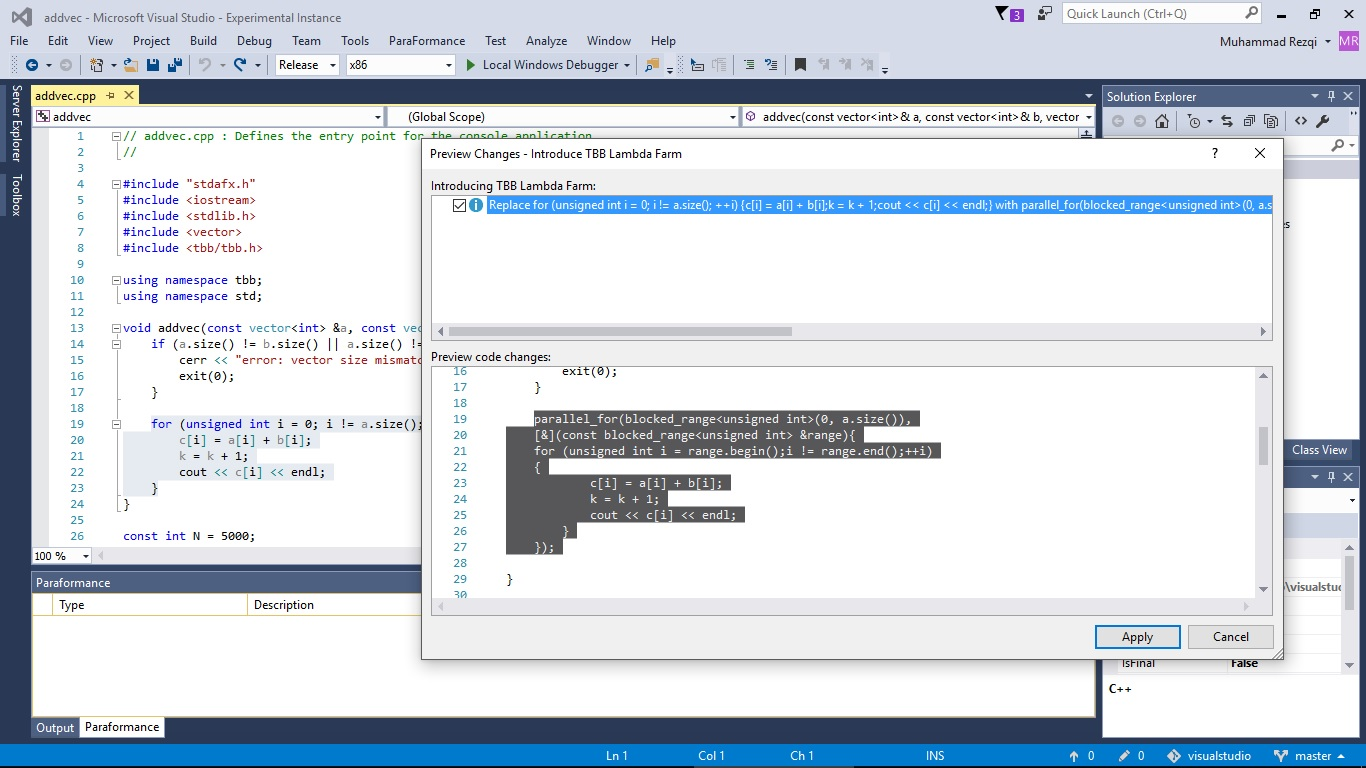
\includegraphics[scale=0.3]{figures/TBBLambda.jpg}
    \caption{The ParaFormance Refactoring tool, introducing a TBB \texttt{parallel-for} into C++ source code, using Visual Studio.}
    \label{fig:paraformance1}
\end{figure}

\subsection{GRPPI}

GrPPI\cite{D24,DBLP:journals/concurrency/AstorgaD0G17} is a parallel pattern interface
which uses C++ template metaprogramming to provide implementations of
a number of parallel patterns.  The GrPPI patterns are generic over a
number of different parallelism models, currently including (at least
partial) support for Posix threads (PThreads), OpenMP, Intel's Thread Building Blocks (TBB), FastFlow, and
CUDA Thrust.  This enables users to write their application without
needing to know the details of a particular model, and to easily
switch between models.  This strategy greatly reduces the load on the programmer.


\subsection{Structure of GrPPI patterns}\label{sec:pattern-structure}

The basic GrPPI model is of a \textit{pipeline} which processes a
stream of data items: items are produced by a \textit{source},
processed by some intermediate components, and then disposed of by a
\textit{sink}. The individual stages can all be executed in parallel,
so that an item can be processed by stage number $n$ at the same time
as the following item is being processed by stage $n-1$ (and the item
after that by stage $n-2$, and so on): see Figure~\ref{pipeline1}.  

There are various types of
intermediate stage, some of which may themselves be carrying out
parallel computations internally.  Pipeline stages are represented by C++
lambda expressions, or by GrPPI constructs containing lambda expressions,
and are supplied as arguments to the GrPPI \texttt{Pipeline} template.

\begin{figure}[!ht]
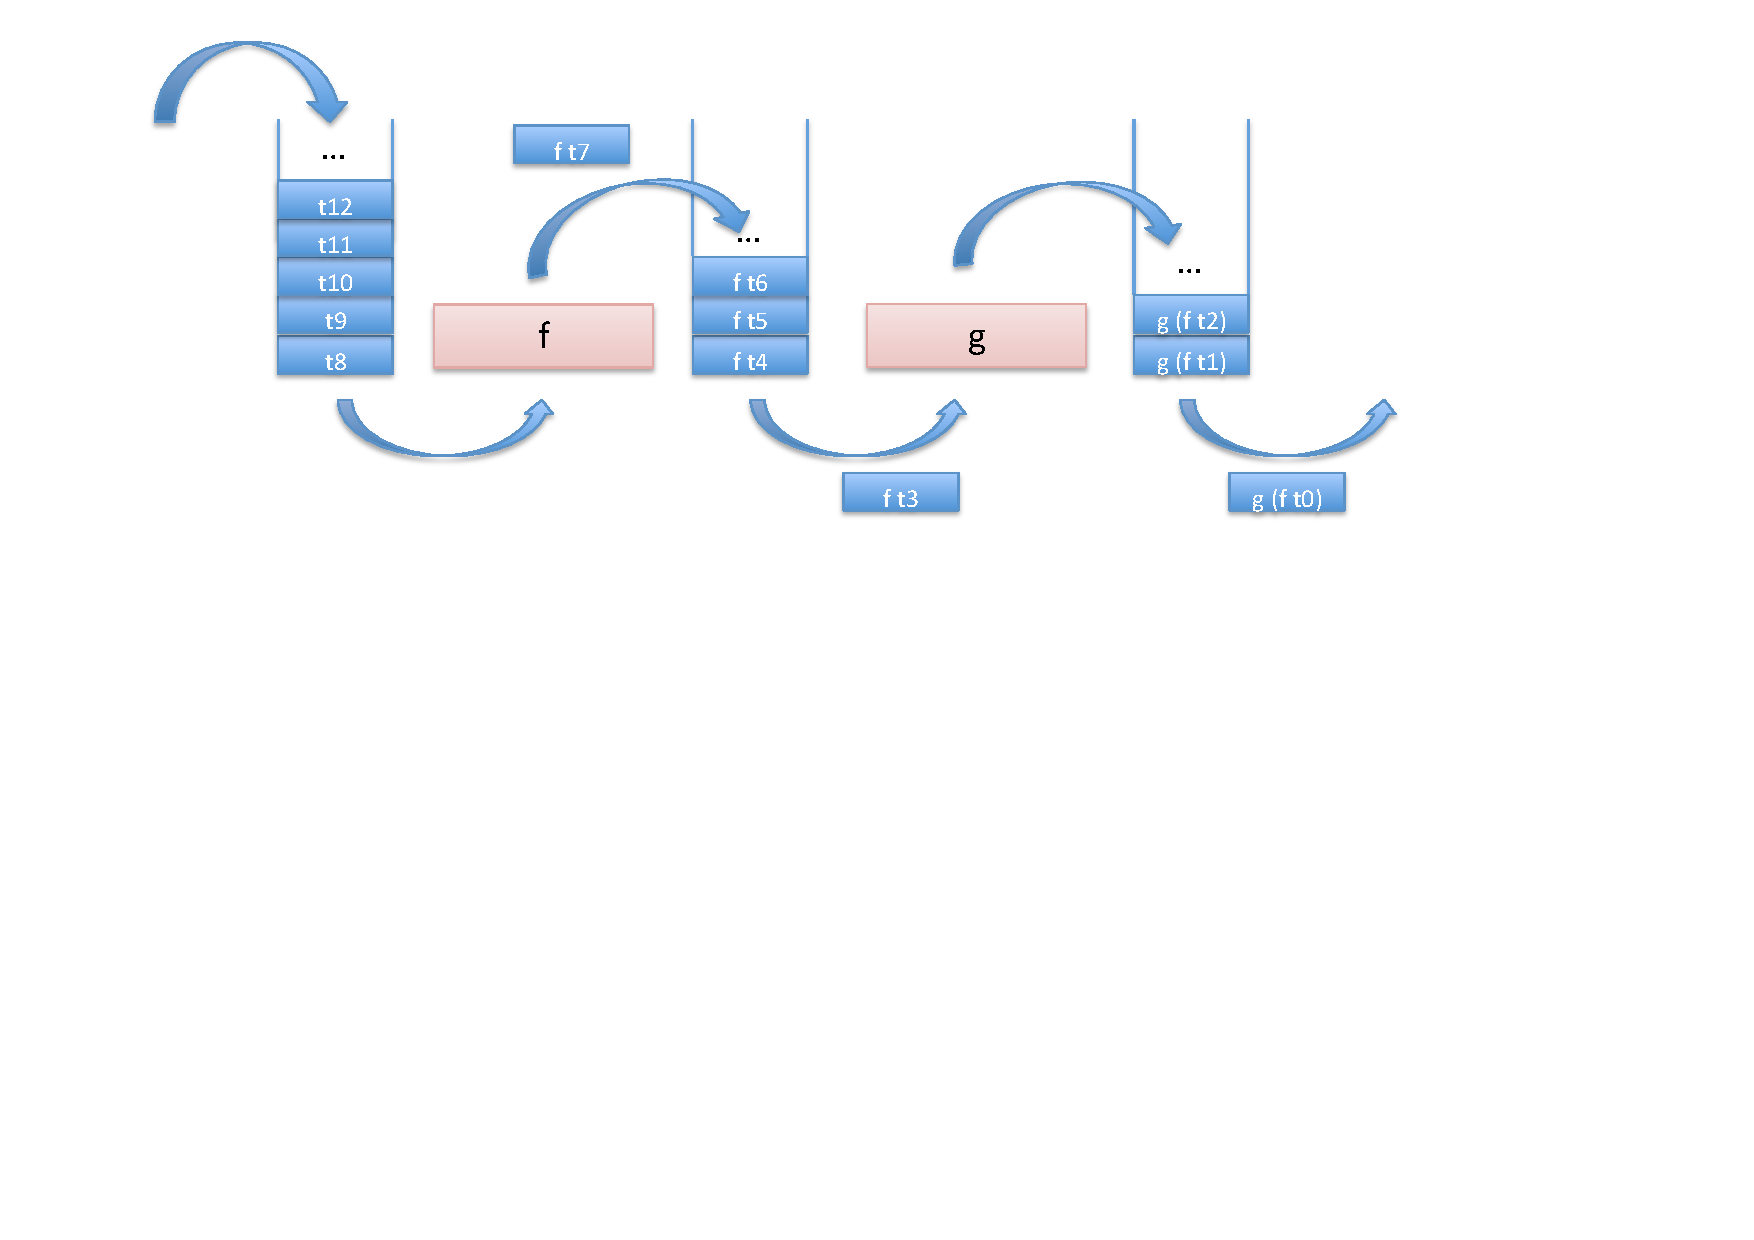
\includegraphics[width=12cm]{figures/pipeline.pdf}

\caption{A Parallel Pipeline Pattern.}
\label{pipeline1}
\end{figure}


\paragraph{Data sources.}  A source produces a stream of items of some type \verb|T|.
The output of the source is in fact of type \verb|optional<T>| so
that the pipeline can tell when the input stream has come to and
end.

%\footnote{See
%  \url{http://en.cppreference.com/w/cpp/utility/optional} for
%  information about the \texttt{optional} type.  This is a proposed
%  extension for C++17 which is not available in most current C++
%  compilers; GrPPI provides its own implementation.}.

\paragraph{Data sinks.}
A sink takes a single item of data and disposes of it in some way, returning \verb|void|.
For example, a sink might write an item to a file, or store it in an array or vector.

\paragraph{Intermediate stages.} GrPPI provides several types of intermediate stage, including:
\begin{itemize}
\item Sequential stages, containing purely sequential code
\item Farms, which can process multiple items in parallel
\item Filters, which can discard items in the input stream based on some predicate
\item Accumulators, which can amalgamate several stream items into a single item for processing by the next stage
\end{itemize}

Pipeline stages are usually represented by C++ lambda expressions,
perhaps wrapped inside GrPPI templates.  A simple example is given
below: this reads a number of integers from a file, squares each one,
and writes the results to \verb|std::cout|. We assume that the
variable \verb|is| is of type \verb|istream| and is associated
with a text file containing a list of integers.

{\scriptsize
\begin{lstlisting}
   parallel_execution_ff p{};
   parallel_execution_ff f{};

   Pipeline(p,
      [&]() {
          int i;
          if (is >> i) return optional<int>(i);
          else return optional<int>();
      },

      Farm(f,
         [&](int k) {
            return k*k;
         }),

      [&](int n) {
         cout << n << endl;
      }
   );
\end{lstlisting}
}

The two \verb|parallel_execution_ff| declarations introduce GrPPI
objects which describe the execution model to be used by 
the parallel pipeline components.  The \verb|ff| part indicates that
the FastFlow execution model should be used; to use OpenMP (say)
instead, one would replace these with \verb|parallel_execution_omp|.

The first stage reads integers from the file and feeds them into the pipeline.
The second stage squares the input items; since it is a \verb|Farm| object,
multiple items are processed in parallel and the results may not be output
in the same order as the inputs.
The final stage prints the squared data items to the standard output stream.


\section{Refactorings for GrPPI}
\label{refactoring_grppi}

In this section we introduce new refactorings implemented in the ParaFormance tool that introduce GrPPI patterns in sequential C++ source code. In this paper we target the \emph{pipeline} and \emph{farm} patterns.

\subsection{Introducing a GrPPI Pipeline}\label{refactoring-interface}

This refactoring converts a C++
\texttt{for} loop into a GrPPI pipeline containing one or more stages
that are executed concurrently to process a sequence of data items
indexed by the loops. We currently support sequential stages that
process a single data item at a time, and farm stages that process
multiple items in parallel. 
% Note that the refactoring imposes the mild
% restriction that the body of the loop must be a compound statement
% enclosed in braces: \texttt{\{...\}}.

% The intention here is that the user selects an initial parallelism model
% but is able to select extra headers to allow the parallelism model to be
% changed later. For example, one could change
% \texttt{parallel\_execution\_native} to
% \texttt{parallel\_} \texttt{execution\_tbb} in the program source; if the TBB
% headers have already been included then no other changes will be
% required in the source. These settings will be remembered between
% invocations of the refactoring, but will be reset to a default if
% Eclipse is restarted. The form also allows the user to enter a name for
% the pipeline: the default is \texttt{pipe} (possibly with a numeric
% suffix to avoid conflicts with other variables which are in scope), but
% any other name can be used.

%Once the form has been completed, the user can select
%either \textit{Preview} to display the changes which will be made,
%or \textit{OK} to perform the changes directly, without a
%preview. They can also press \textit{Cancel} to abandon the process
%and leave the program source unaltered.
%
%Note that for Eclipse to parse and build the refactored code,
%appropriate include paths and compiler options may need to be added to
%the project build configuration.

\subsection{Refactoring strategy}\label{refactoring-strategy}

To refactor a \texttt{for} loop, the loop must be in the form,
% 
% \begin{enumerate}
%\tightlist
% \item
\begin{lstlisting}[mathescape]
for (T x=e1; e2; e3) {$\dots$}
\end{lstlisting}

% \item
%   \lstinline[mathescape]|for (x=e1; e2; e3) {$\dots$}|
% \end{enumerate}
\noindent
% Here \texttt{x} is a variable name and \texttt{T} is a type.
for some variable, \texttt{x}, and type \texttt{T}, where \texttt{T} may be omitted.
As is standard,
\texttt{e1} is an initial value for \texttt{x}, \texttt{e2} is some
bounding condition, and \texttt{e3} is an expression that updates the
value of \texttt{x}. When \texttt{e2} is empty, the
pipeline will run forever. The refactoring requires that \texttt{e3} must not be empty. The
% crucial restriction here is that the 
loop must declare or initialise a
single variable in the initialiser; this variable represents data
items passing through the pipeline.
% 
These patterns enable the refactoring of common types of loop; e.g.
% \begin{itemize}
% \item \lstinline[mathescape]|
\begin{lstlisting}[mathescape]
for (int i=0; i<N; ++i) {
  $\dots$
}
\end{lstlisting}

\noindent
and
\begin{lstlisting}[mathescape]
for (auto i = v.begin(); i != v.end; ++i) {
  $\dots$
}
\end{lstlisting}

\begin{figure}
\centering
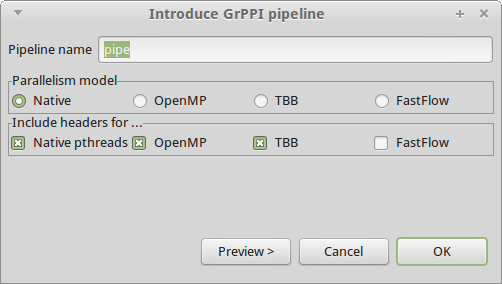
\includegraphics[width=4in]{figures/InputForm.png}
\caption{Input Form for ParaFormance GrPPI Refactorings}
\label{fig:inputform}
\end{figure}

\noindent
The refactoring requires that the body of the \texttt{for} loop is a compound statement enclosed in braces; i.e.\ \texttt{\{\dots\}}; and is dependent upon the existence of pragmas in the loop body that indicate the pipeline stages. These pragmas may be introduced manually by the programmer, or automatically via some tool, which we intend to investigate as part of future work.
% The refactoring 
% Prior to refactoring, the user must manually insert pragmas into the
% body of the loop indicating the pipeline stages (we expect this process to be automated in future work).
These pragmas include:
% 
\begin{itemize}
%\tightlist
\item
  \lstinline|#pragma grppi seq stage|
\item
  \lstinline|#pragma grppi farm stage|
\item
  \lstinline[mathescape]|#pragma grppi farm stage $n$|
\end{itemize}

\noindent
A GrPPI farm stage must specify a number of threads to execute the farm.
By default this is 4, but the pragma can provide an alternative value, $n$, where $n$ is a literal integer or variable name bound to a literal integer.
% , which will be used in the
% refactored code.
% This will usually be a literal integer or a variable
% name, but in fact any trailing text in a \texttt{grppi\ farm\ stage}
% pragma will be inserted directly into the refactored code. There is no
% check of syntactic validity, so it is up to the user to write something
% sensible.
%
It is possible to create a pipeline which consists of a single
farm stage: this is equivalent to running multiple (and possibly all)
iterations of the loop concurrently.

% Once the pragmas have been inserted, the user highlights the
% relevant loop and selects
% \textit{GrPPI\ \textgreater{}\ Introduce\ GrPPI\ Pipeline} in the
% \textit{ParaFormance} menu. A form appears allowing the user to
% enter a name for the pipeline and select the parallelism model (see Figure~\ref{fig:inputform}, shown for Eclipse).



Once invoked, the refactoring requires the programmer to provide: a name for the pattern to be inserted; the model of parallelism, e.g.\ pthreads or TBB; and any additional headers for other modes. This is provided via a form in Eclipse (Figure~\ref{fig:inputform}).
% 
The refactoring procedure creates a GrPPI \lstinline|pipeline| object and
inserts a source object which returns consecutive values for \texttt{x}
in the form of \texttt{optional} items, with an empty value when there
are no data items left.
%
The pipeline stages in the loop body are converted into a sequence of
lambda expressions following the source. If a variable is declared
inside a loop stage but required in a later stage, it will be returned
from the corresponding lambda and passed as an argument to the following
lambda: if there is more than one such variable then they will be
returned packed into a tuple which will then be unpacked into variables
in the next stage.
%
Variables which are declared outside the loop are captured in the lambda
expressions \emph{by reference}, which means that the lambdas can modify
them: this may lead to race conditions.

For example, given the loop
% 
\begin{lstlisting}
for (int i=0; i < SIZE; i++) {
  #pragma grppi seq stage
  xs[i]
}
\end{lstlisting}

\subsection{Safety checking}\label{safety-checking}

The refactoring carries out some simple safety checks. If the loop
body contains a \texttt{return}, \texttt{break}, \texttt{continue},
\texttt{goto}, or \texttt{exit} a fatal error will be issued, since
% these statements
% will either fail to make sense inside the refactored
% code, or could 
can cause an iteration of the loop to terminate when later
iterations have already begun to execute, almost certainly violating the
intended semantics of the loop. Other problems may arise from the fact that the loop body is broken up
into several parts with data being passed between them. For example:
% 
% \begin{itemize}
% \item
  For example, if a large data structure is allocated on the stack (more precisely,
  with automatic storage duration) in one stage and used again in a
  later stage, it will be \emph{copied} as a parameter, which could be
  problematic if the structure is large.
% \item
  Another example occurs when a pointer is created to a stack-allocated variable in one stage and
  then used in a later stage, the data to which it is pointing may have
  changed, or the memory may be in use for something completely
  unrelated.
% \end{itemize}
% 
These checks are not exhaustive and addressing other potential problems is a topic of future work.

%Ultimately the user must be careful not to introduce race conditions or
%other concurrency problems. Work is ongoing to detect these problems
%automatically, but is not yet complete.

\subsection{While loops}\label{while-loops}

Given a general \texttt{while} loop it can be
difficult to decide whether it processes a sequence of items in a manner
suitable for pipelining: for example, the input to one iteration may be
the output of the previous iteration (as would happen in many types of
simulation, where each iteration of a loop represents the evolution of
some system over a single timestep), and this dependence makes the loop
unsuitable for pipelining. However, we have identified a number of
commonly-occurring patterns which are plausible candidates for
pipelining and which the tool will refactor.
% 
\begin{enumerate}
\def\labelenumi{\arabic{enumi}.}
%\tightlist
\item
  \lstinline[mathescape]|while (x=e) {$\dots$}|
\item
  \lstinline[mathescape]|while ((x=e1)  op e2) {$\dots$}|
\item
  \lstinline[mathescape]|while (obj >> x) {$\dots$}|
\end{enumerate}

% \begin{itemize}
% \item 
\noindent
In case 1, we assume that \texttt{x} is being given a new value by some
expression \texttt{e} which presumably performs some side-effect; for
example \texttt{while\ (x=*p++)\ ...}. EXAMPLE
% 
% \item 
In case 2, we again assume that \texttt{x} is being supplied with new
values by \texttt{e1} and the value is being compared with e2 using some
binary operator \texttt{op}; for example
\texttt{while\ ((x=getc(stream))\ \textgreater{}=\ 0)\ ...} EXAMPLE
% 
% \item 
In case 3, we assume that the \texttt{\textgreater{}\textgreater{}}
operator is supplying new values from a stream or some other type of
object. This allows us to handle common idioms such as
\texttt{while\ (std::cin\ \textgreater{}\textgreater{}\ x)\ ...}. EXAMPLE
% \end{itemize}

% As before, suitable pragmas should be inserted in the loop body and then
% \textit{Introduce\ GrPPI\ Pipeline} selected.
%
%We emphasise that this feature is experimental and should be used with
%care: it is quite possible that problems may arise which we have not
%anticipated. Moreover, the plugin is not performing full dependency
%analysis (although reports of race conditions on the loop variable are a
%clear danger signal), so it is possible that the refactoring may not
%preserve the semantics of the loop. We hope to introduce more
%comprehensive safety checks in future versions of the tool.

\section{Safety Checking}
\begin{figure}
\centering
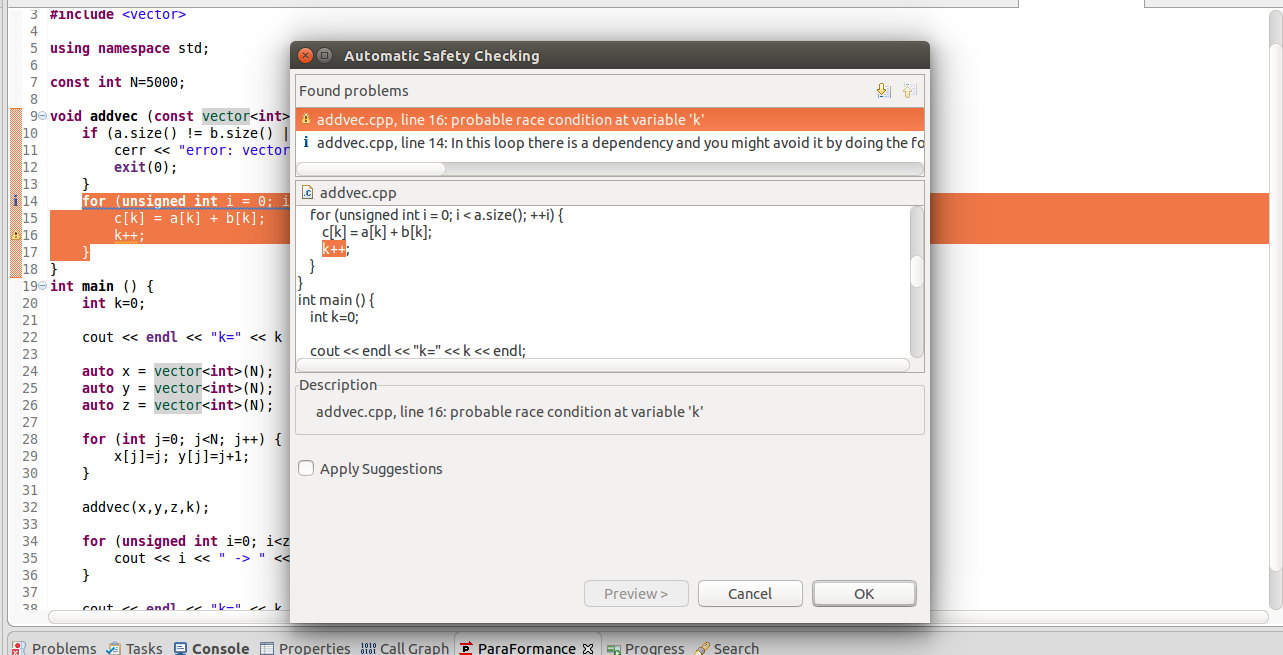
\includegraphics[scale=0.26]{figures/pf-safety-auto-dialog.png}
\caption{The ParaFormance Safety Checking View in Eclipse}
\label{fig:safety1}
\end{figure}

The safety check is a fundamental feature in the ParaFormance tool. In this check, a static check is carried out to ensure the code being refactored is safe for parallelisation. Validity means the code is free from dependencies, side effects (such as writing to a global state), or contains code that may interfere with the parallel logic.
%
The refactorings produced by the ParaFormance tool should preserve the correctness of the functional semantics of the C++ program. This means that when given the same input value(s), the program should produce the same output value(s) before and after a refactoring, up to a given ordering.
%
Safety checking does not require the application to be parallelised before proceeding and can run on sequential code. This check ensures a lack of race conditions, deadlocks and other problems that may affect safety. Moreover, this check may introduce additional refactorings to remove/repair these problems. 
%
Figure~\ref{fig:safety1} shows the safety checking feature integrated into ParaFormance; here, a report of safety errors are reported to the user, which the tool has found by analysing the source code. The filename, line numbers and a detailed description are given for each safety error reported. In some cases, a suggestion of how to fix the safety issue is also given. Safety checking is able to capture and detect a wide range of cases. These cases include (but are not limited to):

\begin{itemize}
\item \textbf{Race conditions:} Updating global, static, or free variables causes race conditions in threaded code. Such conditions are captured by the checker with context details. Moreover, a stack trace of function calls is provided when the detected conditions are introduced inside invoked function(s).

An example of race condition is as follows:
\begin{lstlisting}[label=code:filtering_generated,caption={Race Condition}]
int x = ...;
...
for(int i=0; i<MAX;i++){
     ...
     x = x + i;
     ...
}
\end{lstlisting}
Here, updating variable \texttt{x} is a race condition when there are many threads trying to access that variable.

\item \textbf{Object state}: Updating the member fields of objects is problematic in multithreaded programming. This updates the state of the object in the threaded code. Also, the state of the object may be updated when calling overloaded operations such as \texttt{+=}.

\begin{lstlisting}[label=code:filtering_generated,caption={Object State}]
class A {
    public:
        A& operator+=(const A &x) {
            //do_something();
            return *this;
        }
    };
    void funOperator () {
        A x, y;
        for(int i=0;i<10;i++){
            x += y;
        }
    }
}
\end{lstlisting}    
    
Here, the safety checker reports a safety warning saying that there is a probable change in the state of the object \texttt{x} at Line 11.

\item \textbf{Accessing pointers:} The safety checker is able to track all non-safe updates to pointers shared amongst many threads. Also, when there are many references/pointers having access to a value, modifying that value by one thread is problematic. In general, any update to a shared reference/pointer or the content of that reference (variable, pointer or function reference) can be captured.

\begin{lstlisting}[label=code:filtering_generated,caption={Object State}]
 int test_alias(){
        int x = 10;
        for(int i=0;i<20;i++){
            int *p = &x;
            (*p) = (*p) + i;
            //...
        }
    }
\end{lstlisting}

In this example, the pointer \texttt{p} is declared in the loop so it is local variable but it is pointing to stack-allocated variable \texttt{x} so modifying this pointer causes a race condition. using references is also incurring safety problems.

\item \textbf{IO/Streams:} Updating and writing to files, printing to the screen and reading in data are generally considered to be unsafe. The tool highlights any call to the iostream as being unsafe. An example is \texttt{std::cout}.

\begin{lstlisting}[label=code:filtering_generated,caption={IO/Streams}]
An example is std::cout.
    #include <iostream>
    const int L = 0;const int U = 20;
    void fun_cout(){
        for(int I = 0; I < U; I++){
            //...
            std::cout << I;
            //...
        }
    }
\end{lstlisting}

\item \textbf{STL containers:} In C++, there is a set of containers can be used for storing items and doing some operations. These containers have some member functions that are non-thread safe. The tool warns the user about the usage of such functions.

\begin{lstlisting}[label=code:filtering_generated,caption={STL Containers}]
#include <vector>
    void test_stl() {
        std::vector<int> v;
        for (int i = 0; i<10;i++) {
            //...
            v.push_back(i);
            //...
        }
    }
\end{lstlisting}

\item \textbf{Function calls:} When a function is called in the main loop, the safety checker still parses and capture any possible data race. If a data race is detected, the issued warning lists the stack trace stating the all function calls leading to that race case.	
\end{itemize}

\begin{lstlisting}[label=code:filtering_generated,caption={Function Calls}]
int global = 0;
void fun_calls(int &ref,int *pointer, int value){
    global++;
    ref++;
    (*pointer)++;
    value++;
}
int main_fun_call(){
    int x = 10;int *p = &x;int *q = p;
    for(int i=0; i < 50;i++){
       fun_calls(x, &x, x);
    }
}
\end{lstlisting}    
   
Recursive calls are also parsed.

\begin{lstlisting}[label=code:filtering_generated,caption={Recursive Function Calls}]
int total;
void sum(int n){
    if(n == 0) return;
    total += n;
    sum(n-1);
}
void fun_call_recursive(){
    for(int i=0;i<10;i++){
        sum(i);
    }
}
\end{lstlisting}

\section{Related Work}

% In our previous work, we pioneered refactoring to introduce parallelism~\cite{rpl},where sequential code is transformed to introduce instances of parallel patterns. We have shown that this can lead to excellent speedups of the resulting code.

% \begin{itemize}
% \item Refactoring to introduce parallelism
%     \begin{itemize}
%     \item RPL [C++]
%     \item Agricultural Reform [C++]
%     \item Cost-Directed Refactoring, Paraphrasing: Generating Parallel \&c., Safe Concurrency Introduction, (\& Using Program Shaping) [Erlang]
%     \item Stream Parallel Skeleton Optimisation (Aldinucci) [Rewrites]
%     \item Optimisation Rules for Programming with Collective Operations (Gorlatch) [Rewrites]
%     \item Polyhedral model
%     \end{itemize}
% \item GrPPI~\cite{DBLP:journals/concurrency/AstorgaD0G17} \& pattern libraries
%     \begin{itemize}
%     \item TBB
%     \item Microsoft PPL
%     \item FastFlow
%     \item OpenMP
%     \item Thrust (CUDA/OpenCL)
%     \item SYCL (CUDA/OpenCL)
%     \item RaftLib
%     \item Fusion Embedded Skeleton Library (Matsuzaki)
%     \item Lapedo (CPU \& GPU Mix) [Erlang]
%     \end{itemize}
% \end{itemize}


Refactoring has roots in Burstall and Darlington's fold/unfold system~\cite{darlington77}, and has been applied to a wide range of applications as an approach to program transformation~\cite{mens_refactoring}, with refactoring tools a feature of popular IDEs including, \textit{i.a.}, Eclipse~\cite{EclipseWeb} and Visual Studio~\cite{VisualStudioWeb}.
Previous work on parallelisation \textit{via} refactoring has primarily focussed on the introduction and manipulation of parallel pattern libraries in C++~\cite{brownagricultural,DBLP:conf/pdp/JanjicBMHDAG16} and Erlang~\cite{hlpp,DBLP:journals/cai/BarwellBHTB16}.

Parallel design patterns, or algorithmic skeletons, were suggested as solution to the difficulties presented by low-level approaches~\cite{Asanovic:2009:VPC,DBLP:journals/spe/Gonzalez-VelezL10}.
A range of pattern/skeleton implementations have been developed for a number of programming languages; these include: RPL~\cite{DBLP:conf/pdp/JanjicBMHDAG16}; Feldspar~\cite{DBLP:conf/ifl/AxelssonCSSEP10}; FastFlow~\cite{DBLP:journals/mis/JinLWY15}; Microsoft's Pattern Parallel Library~\cite{ACM:book/msoft/CampbellM11}; and Intel's Threading Building Blocks (TBB) library~\cite{DBLP:reference/parallel/X11pz}.
Since patterns are well-defined, rewrites can be used to automatically explore the space of equivalent pattern, e.g. optimising for performance~\cite{DBLP:conf/europar/MatsuzakiKIHA04,DBLP:conf/ipps/GorlatchWL99} or generating optimised code as part of a DSL~\cite{DBLP:conf/dagstuhl/Gorlatch03}. Moreover, since patterns are architecture-agnostic, patterns have been similarly implemented for multiple architectures~\cite{DBLP:conf/cgo/HagedornSSGD18,DBLP:conf/parco/ReyesL15}.

This introduces a level of specialisation, and the possibility of choice between pattern implementations. Conversely, GrPPI~\cite{DBLP:journals/concurrency/AstorgaD0G17} is capable of invoking other libraries, and is thereby able to take advantage of the specialisations that they present without potentially labourious reimplementation.


Elsewhere, approaches to automatic parallelisation have primarily focussed on the transformation of loops. From early approaches in Fortran~\cite{DBLP:journals/cacm/Lamport74}, to more recent attempts with the polyhedral model~\cite{DBLP:conf/ppopp/AncourtI91}. Whilst fully automatic approaches simplify the parallelisation process for the programmer by removing the programmer from the process, such approaches can be very specific in both the code to which they can be applied. Conversely, programmer-in-the-loop approaches, such as refactoring, allow the programmer to employ their knowledge about both code and parallelism.

Similar to our approach, Dig \textit{et al.}~\cite{dig} use refactoring to introduce parallelism in Java. However, unlike our approach Dig \textit{et al.} introduce low-level Java concurrency primitives instead of patterns. More recently,  Radoi and Dig consider data races in Java for parallelism, a key aspect of safety checking~\cite{DBLP:journals/tosem/RadoiD15}. Other safety checking aspects are covered by work on deadlock detection~\cite{DBLP:journals/tse/Corbett96}.


\section{Evaluation}

\subsection{Matrix Multiplication}
\noindent Matrix multiplication is one of the most commonly used simple parallel benchmark that demonstrates the use of \emph{farm} pattern. Here, our baseline hand-tuned parallel version multiplies two $n \times n$ matrices by assigning a separate thread to multiplying each row of the first matrix with the complete second matrix. This is more coarse-grained version of the standard benchmark where a separate thread is assigned to multiplication of each row of the first matrix with each colum of the second matrix. The relevant parts of the sequential and hand-tuned parallel versions are given in Figure~\ref{fig:baselineMatMult}

\begin{figure}[t]
\centering
\subfigure[OpenMP] {
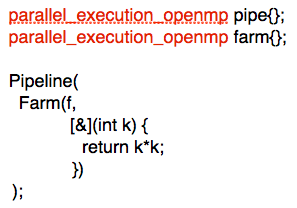
\includegraphics[width=0.35\textwidth]{GrPPIExampleOpenMP.png}
 \label{fig:grppiExampleOpenMP}}
 \subfigure[Intel TBB] {
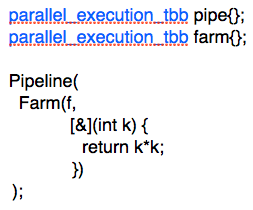
\includegraphics[width=0.30\textwidth]{GrPPIExampleTBB.png}
 \label{fig:grppiExampleTBB} 
  }
\caption{Sequential and \emph{pthreads} parallel Matrix Multiplication versions.}
\label{fig:baselineMatMult}
\end{figure}





\subsection{Railway Diagnostic System}

eRDM is a dynamic railway diagnostic system, supplied by EvoPro Innovations, Hungary. The eRDM is able to measure the load of each wheel, axle and carriage of the train passing over the system at operating speed. The system also provides diagnostic features; it is able to detect unbalanced rail-cars, wheel flat spots, damaged boogies and suspension problems. Thus the system allows real-time freight transportation monitoring, helps increasing railway transportation safety and reducing rail/carriage maintenance costs. The hierarchy of the system can be seen in Figure \ref{fig:erdm_sysoverview}.

\begin{figure}[!ht]
\centering
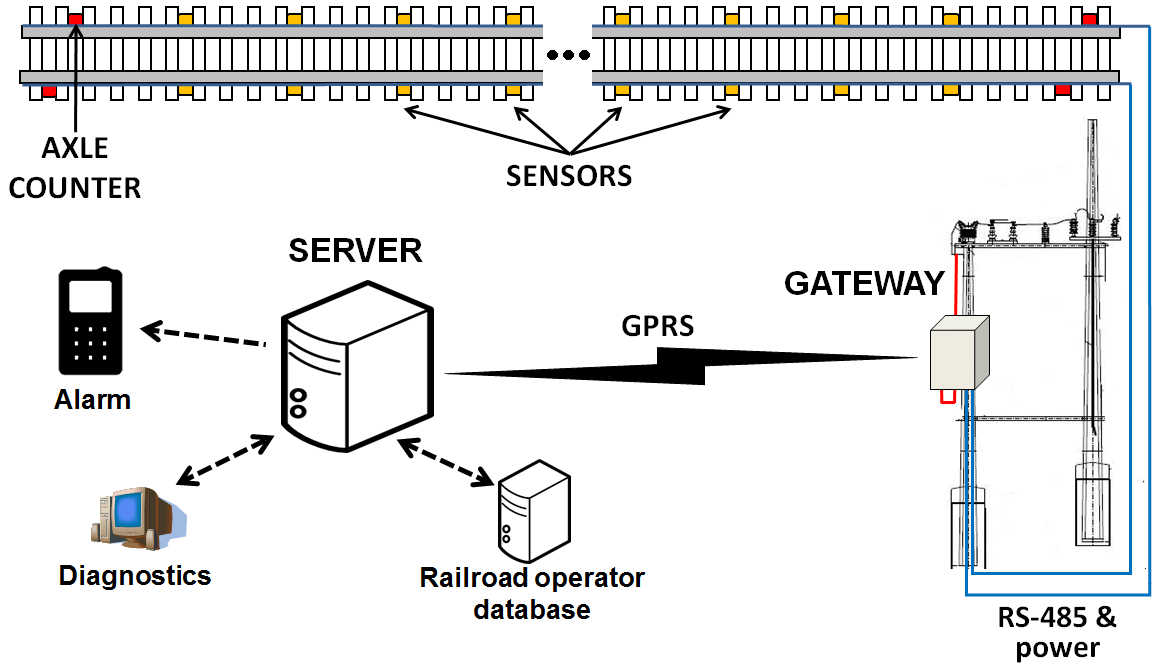
\includegraphics[scale=0.4]{figures/erdm_sysoverview.png}
\caption{ERDM system hierarchy}
\label{fig:erdm_sysoverview}
\end{figure}

\subsubsection{Experimental Setup for eRDM}

The following hardware was used to measure the results for eRDM.
\begin{itemize}
	\item Xeon Server (48 CPU-cores, 2816 GPU-cores) with 2x Intel Xeon E5-2695 v2 CPU (x86) (30M Cache, 2.40 GHz) (12 physical cores each, i. e. 48 cores in total by HyperThreading) and 8x16 GB of DDR3 1600 MHz memory.
	\item Nvidia Jetson TK1 board (4 CPU-cores, 192 GPU-cores) with NVIDIA 4-Plus-1 Quad-Core ARM Cortex-A15 CPU (2.32 GHz), and 2 GB of DDR3L 933MHz memory.
	\item Gizmo 2 board (2 CPU-cores, 80 GPU-cores), with AMD GX-210HA Dual-Core CPU (x86) (1M Cache, 1 GHz), i. e. 2 cores, and 1GB of DDR3 1600 MHz memory.
\end{itemize}
An important modification in the Gizmo 2 hardware is that we replaced the SD card with an SSD to reach higher performance. The SD card used as permanent storage represented a serious performance bottleneck and lead to quite poor performance in D6.4; all the results presented in this deliverable were obtained using the improved configuration.

\subsubsection{Refactoring eRDM}

Apply the GRPPI refactorings from Section~\ref{refactoring_grppi}, the outer loop of the original kernel code was parallelized by applying a pipeline with a farm-based processing stage for the bulk of the code. The generated code did not require any further refinements, it could be directly compiled and executed. Moreover, there was no need to restructure the code manually before transformation, only the pragmas have been inserted as preparation. 

\paragraph{Inserting pragma statements into the original code}
This preparation step included inserting two pragmas into the original kernel code. These statements inform the ParaFormance plugin as to what type of structure has to be generated from the original source. The relevant code section after inserting pragmas is shown on Listing \ref{code:filtering_with_pragmas}.

\begin{small}
\begin{lstlisting}[label=code:filtering_with_pragmas,caption={Original eRDM kernel code with pragma statements}]
unsigned int numOfThreads = 8;

const float* bp_coeffs = RCBProc::bandpass_coefs;
const float* hil_coeffs = RCBProc::hilbert_coefs;
unsigned int numOfCoeffs = RCBProc::filterLength;

//filtering
for (unsigned int rcbIdx = 0; rcbIdx < numberOfRCBs; rcbIdx++) {
#pragma grppi seq stage

   float* inputSignal = RCBs[rcbIdx].rcbProc.rawData.data();
   float* filteredSignal = RCBs[rcbIdx].rcbProc.filteredData.data();
   unsigned int numOfSamples = RCBs[rcbIdx].rcbProc.rawData.size();

#pragma grppi farm stage numOfThreads
   for (unsigned int sampIdx = 0; sampIdx < numOfSamples; sampIdx++) {
       filteredSignal[sampIdx] = 0.0f;
       if (sampIdx >= numOfCoeffs - 1) {
         float bp_temp = 0.0;
         float hil_temp = 0.0;
         for (unsigned int coeffIdx = 0; coeffIdx < numOfCoeffs; coeffIdx++) {
            bp_temp += bp_coeffs[coeffIdx] * inputSignal[sampIdx - coeffIdx];
            hil_temp += hil_coeffs[coeffIdx] * inputSignal[sampIdx - coeffIdx];
         }
         filteredSignal[sampIdx] = sqrt(bp_temp * bp_temp + hil_temp * hil_temp);
       }
   }
}


\end{lstlisting}
\end{small}


\paragraph{Refactoring using ParaFormance and GRPPI}
After inserting pragmas, we highlighted the outer for loop area then selected the GrPPI option of the ParaFormance menu and clicked \emph{Introduce GrPPI Pipeline}. In the configuration window everything was left default; that is, we used the Native parallelism model similarly to the manual case. Finally the code generation process was launched. The result of it is shown on Listing \ref{code:filtering_generated}.

The generated pipeline consists of two stages. Input of the pipeline is the index of the sensor to be processed. The first stage implements a simple preparation step, it justs sets the input/output data pointers according to the sensor index. The second stage of the pipeline is a farm containing the actual processing code, which thus will be executed in parallel for the different sensors by the specified amount of worker threads.

\begin{small}
\begin{lstlisting}[label=code:filtering_generated,caption={eRDM refactored using ParaFormance}]
unsigned int numOfThreads = 8;

const float* bp_coeffs = RCBProc::bandpass_coefs;
const float* hil_coeffs = RCBProc::hilbert_coefs;
unsigned int numOfCoeffs = RCBProc::filterLength;

//BENCHMARK START
double startTime = Utils::getTimeSec();

unsigned int rcbIdx = 0;
parallel_execution_native pipe { };

//filtering
pipeline(pipe,
// -------- source ---------- //
    [&]() {
       if (rcbIdx < numberOfRCBs) {
          auto _r = rcbIdx;
          rcbIdx++;
          return std::experimental::optional<unsigned int>(_r);
          } else return std::experimental::optional<unsigned int>();
     },
     // -------- stage 1 ---------- //
     [&](unsigned int rcbIdx) {
        float* inputSignal = RCBs[rcbIdx].rcbProc.rawData.data();
        float* filteredSignal = RCBs[rcbIdx].rcbProc.filteredData.data();
        unsigned int numOfSamples = RCBs[rcbIdx].rcbProc.rawData.size();
        return std::make_tuple(numOfSamples, filteredSignal, inputSignal);
      },
      // -------- stage 2 ---------- //
     farm(numOfThreads,
     [&](std::tuple<unsigned int, float *, float *> _args) {
        unsigned int numOfSamples = std::get<0>(_args);
        float * filteredSignal = std::get<1>(_args);
        float * inputSignal = std::get<2>(_args);
        for (unsigned int sampIdx = 0; sampIdx < numOfSamples; sampIdx++) {
        filteredSignal[sampIdx] = 0.0f;
           if (sampIdx >= numOfCoeffs - 1) {
             float bp_temp = 0.0;
             float hil_temp = 0.0;
             for (unsigned int coeffIdx = 0; coeffIdx < numOfCoeffs; coeffIdx++) {
                bp_temp += bp_coeffs[coeffIdx] * inputSignal[sampIdx - coeffIdx];
                hil_temp += hil_coeffs[coeffIdx] * inputSignal[sampIdx - coeffIdx];
             }
             filteredSignal[sampIdx] = sqrt(bp_temp * bp_temp + hil_temp * hil_temp);
         }
     }
     return;
}));

\end{lstlisting}
\end{small}

%\subsection{Number of threads in the farm pattern}
%
%In order to get the best execution time on the given hardware platform we performed some experiments with a different number of worker threads applied. Figure \ref{fig:erdm_res_grppi_pipe} shows the execution times of the kernel code for various number of threads, for various train lengths on the Xeon Server. In case of the Xeon Server it seems that applying more than 8 worker threads does not give any real further speedup. However, for the parallel versions described in D6.4 we used 16 workers; therefore we applied 16 as the thread number in D6.6 so that a fair and consistent comparison can be made. The Jetson board has 4 CPU cores, so we specified 4 worker in this case. Following this rule 2 workers were used in case of the double-core Gizmo 2 platform.
%
%\begin{figure}[ht]
%	\centering
%	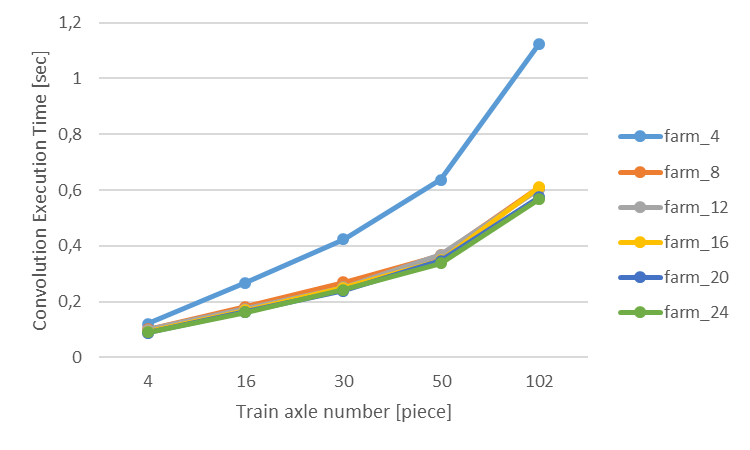
\includegraphics[width=0.9\linewidth]{figures/cpu_grppi_farms_server.png}
%	\caption{GrPPI pipeline with farm using different thread numbers on Xeon Server}
%	\label{fig:erdm_res_grppi_pipe}
%\end{figure}

\subsubsection{Measurement results}

Figure \ref{fig:erdm_res_grppi_pipe_xeon} shows the measured execution times on the Xeon Server. Similarly, these results are presented in figures \ref{fig:erdm_res_grppi_pipe_jetson} and \ref{fig:erdm_res_grppi_pipe_gizmo2}. On the Xeon Server an average speedup of x6.07 could be obtained with the automatically generated GrPPI pipeline code over the sequential one, with a maximal speedup of x7.26 for the 102 axle train. In case of the Jetson board the average speedup was x3.45. The Gizmo 2 platform reached averagely x1.98 faster execution in case of the pipeline-based solution compared to the sequential version. In contrast to the map-based solution the achieved speedup highly depends on the input data size (number of axles) in this case, especially on the Xeon Server, where the speedup was only x4.29 for a 4 axle train. 
\begin{figure}[t]
\centering
\subfigure[GrPPI Pipeline with Farm results of Xeon Server for eRDM] {
\begin{tikzpicture}[thick,scale=0.65]
\begin{axis}[
  mark size=0.6mm,
  cycle list={
    {blue,mark=star},
    {red,mark=diamond},
    {brown!60!black,mark=triangle},
    {blue,dashed,mark=star},
    {red,dashed,mark=diamond},
    {brown!60!black,dashed,mark=triangle},
  },
  legend style={
    font=\small,
    cells={anchor=west},
  },
  legend pos= north west,
  enlargelimits,
  xtick={4,16,30,50,102},
   ytick={0, 0.5, 1, 1.5, 2, 2.5, 3, 3.5, 4, 4.5, 5},
   ymax=5,
   xlabel=Train Axle Number (pieces),
   ylabel=Convolution Execution Time (sec),
  % title=Speedups for Ant Colony
   ]
   \addplot table[x index=0,y index=1] {results/cpu_meas.txt};
   \addplot table[x index=0,y index=1] {results/grppi_meas_results.txt};
   \legend{Manual GrPPI, Refactored GrPPI}
\end{axis} 
 \end{tikzpicture}
 \label{fig:erdm_res_grppi_pipe_xeon}}
 \subfigure[GrPPI pipeline with farm results on Jetson board for eRDM] {
\begin{tikzpicture}[thick,scale=0.65]
\begin{axis}[
  mark size=0.6mm,
  cycle list={
    {blue,mark=star},
    {red,mark=diamond},
    {brown!60!black,mark=triangle},
    {blue,dashed,mark=star},
    {red,dashed,mark=diamond},
    {brown!60!black,dashed,mark=triangle},
  },
  legend style={
    font=\small,
    cells={anchor=west},
  },
  legend pos= north west,
  enlargelimits,
  xtick={4,16,30,50,102},
   ytick={0, 1,2,3,4,5,6,7,8},
   ymax=8,
   xlabel=Train Axle Number (pieces),
   ylabel=Convolution Execution Time (sec),
  % title=Speedups for Ant Colony
   ]
   \addplot table[x index=0,y index=1] {results/cpu_meas_jetson.txt};
   \addplot table[x index=0,y index=1] {results/grppi_meas_results_jetson.txt};
   \legend{Manual GrPPI, Refactored GrPPI}
\end{axis} 
 \end{tikzpicture}
 \label{fig:erdm_res_grppi_pipe_jetson}}
  \subfigure[GrPPI pipeline with farm results on Gizmo 2 board for eRDM] {
\begin{tikzpicture}[thick,scale=0.65]
\begin{axis}[
  mark size=0.6mm,
  cycle list={
    {blue,mark=star},
    {red,mark=diamond},
    {brown!60!black,mark=triangle},
    {blue,dashed,mark=star},
    {red,dashed,mark=diamond},
    {brown!60!black,dashed,mark=triangle},
  },
  legend style={
    font=\small,
    cells={anchor=west},
  },
  legend pos= north west,
  enlargelimits,
  xtick={4,16,30,50,102},
   ytick={0, 5, 10, 15, 20, 25},
   ymax=25,
   xlabel=Train Axle Number (pieces),
   ylabel=Convolution Execution Time (sec),
  % title=Speedups for Ant Colony
   ]
   \addplot table[x index=0,y index=1] {results/cpu_meas_gizmo.txt};
   \addplot table[x index=0,y index=1] {results/grppi_meas_results_gizmo.txt};
   \legend{Manual GrPPI, Refactored GrPPI}
\end{axis} 
 \end{tikzpicture}
\label{fig:erdm_res_grppi_pipe_gizmo2}}


\caption{Results for refactored versus manual GrPPI implementations of the eRDM use case}
\end{figure}


%\begin{figure}[!ht]
%	\centering
%	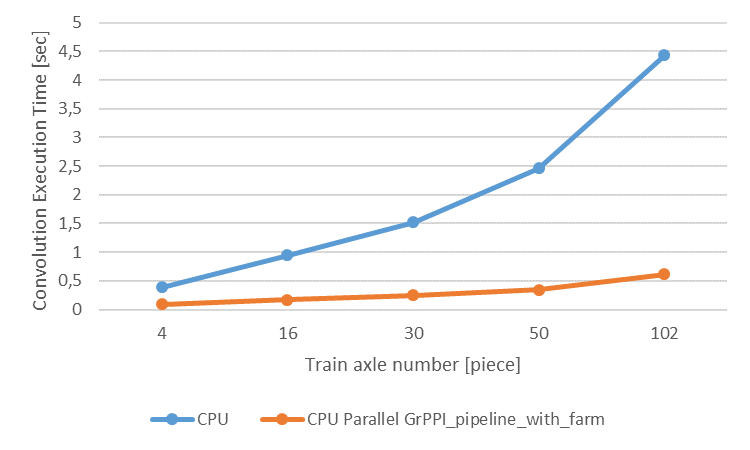
\includegraphics[width=0.9\linewidth]{figures/cpu_grppi_pipe_farm_server.png}
%	\caption{GrPPI pipeline with farm results on Xeon Server}
%	\label{fig:erdm_res_grppi_pipe_xeon}
%\end{figure}
%\begin{figure}[!ht]
%	\centering
%	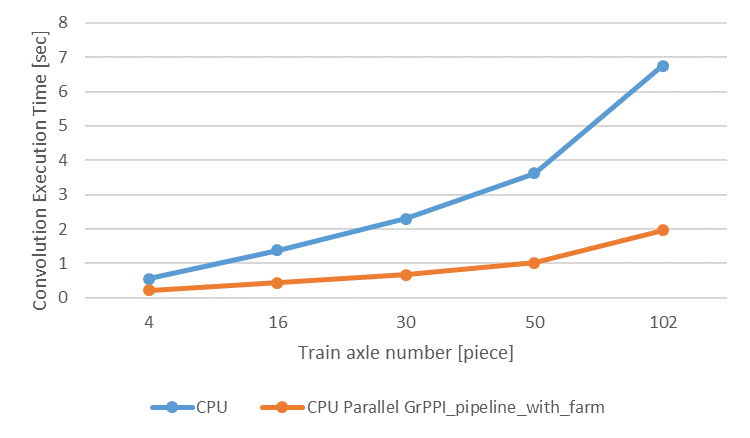
\includegraphics[width=0.9\linewidth]{figures/cpu_grppi_pipe_farm_jetson.png}
%	\caption{GrPPI pipeline with farm results on Jetson board}
%	\label{fig:erdm_res_grppi_pipe_jetson}
%\end{figure}
%\vfill\clearpage
%\begin{figure}[!ht]
%	\centering
%	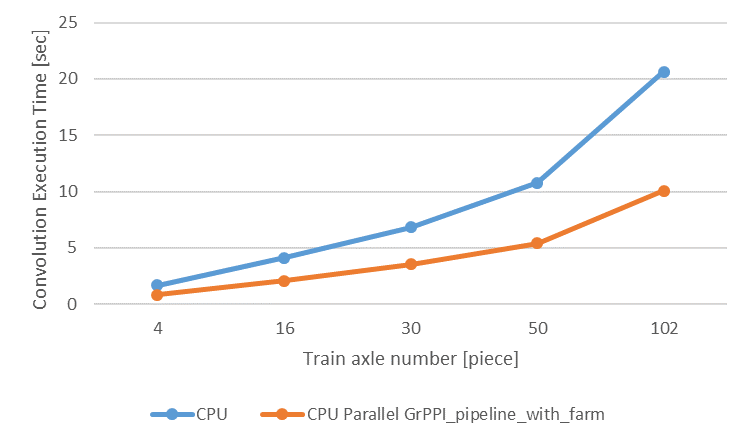
\includegraphics[width=0.9\linewidth]{figures/cpu_grppi_pipe_farm_gizmo2.png}
%	\caption{GrPPI pipeline with farm results on Gizmo 2 board}
%	\label{fig:erdm_res_grppi_pipe_gizmo2}
%\end{figure}






\section{Conclusions and Future Work}



%\begin{acknowledgements}
%If you'd like to thank anyone, place your comments here
%and remove the percent signs.
%\end{acknowledgements}

% BibTeX users please use one of
% \bibliographystyle{spbasic}      % basic style, author-year citations
\bibliographystyle{spmpsci}      % mathematics and physical sciences
%\bibliographystyle{spphys}       % APS-like style for physics
\bibliography{hlpp,RePhrase,rephrase2}   % name your BibTeX data base


\end{document}
% end of file template.tex

